% Options for packages loaded elsewhere
\PassOptionsToPackage{unicode}{hyperref}
\PassOptionsToPackage{hyphens}{url}
%
\documentclass[
]{article}
\usepackage{amsmath,amssymb}
\usepackage{iftex}
\ifPDFTeX
  \usepackage[T1]{fontenc}
  \usepackage[utf8]{inputenc}
  \usepackage{textcomp} % provide euro and other symbols
\else % if luatex or xetex
  \usepackage{unicode-math} % this also loads fontspec
  \defaultfontfeatures{Scale=MatchLowercase}
  \defaultfontfeatures[\rmfamily]{Ligatures=TeX,Scale=1}
\fi
\usepackage{lmodern}
\ifPDFTeX\else
  % xetex/luatex font selection
\fi
% Use upquote if available, for straight quotes in verbatim environments
\IfFileExists{upquote.sty}{\usepackage{upquote}}{}
\IfFileExists{microtype.sty}{% use microtype if available
  \usepackage[]{microtype}
  \UseMicrotypeSet[protrusion]{basicmath} % disable protrusion for tt fonts
}{}
\makeatletter
\@ifundefined{KOMAClassName}{% if non-KOMA class
  \IfFileExists{parskip.sty}{%
    \usepackage{parskip}
  }{% else
    \setlength{\parindent}{0pt}
    \setlength{\parskip}{6pt plus 2pt minus 1pt}}
}{% if KOMA class
  \KOMAoptions{parskip=half}}
\makeatother
\usepackage{xcolor}
\usepackage[margin=1in]{geometry}
\usepackage{color}
\usepackage{fancyvrb}
\newcommand{\VerbBar}{|}
\newcommand{\VERB}{\Verb[commandchars=\\\{\}]}
\DefineVerbatimEnvironment{Highlighting}{Verbatim}{commandchars=\\\{\}}
% Add ',fontsize=\small' for more characters per line
\usepackage{framed}
\definecolor{shadecolor}{RGB}{248,248,248}
\newenvironment{Shaded}{\begin{snugshade}}{\end{snugshade}}
\newcommand{\AlertTok}[1]{\textcolor[rgb]{0.94,0.16,0.16}{#1}}
\newcommand{\AnnotationTok}[1]{\textcolor[rgb]{0.56,0.35,0.01}{\textbf{\textit{#1}}}}
\newcommand{\AttributeTok}[1]{\textcolor[rgb]{0.13,0.29,0.53}{#1}}
\newcommand{\BaseNTok}[1]{\textcolor[rgb]{0.00,0.00,0.81}{#1}}
\newcommand{\BuiltInTok}[1]{#1}
\newcommand{\CharTok}[1]{\textcolor[rgb]{0.31,0.60,0.02}{#1}}
\newcommand{\CommentTok}[1]{\textcolor[rgb]{0.56,0.35,0.01}{\textit{#1}}}
\newcommand{\CommentVarTok}[1]{\textcolor[rgb]{0.56,0.35,0.01}{\textbf{\textit{#1}}}}
\newcommand{\ConstantTok}[1]{\textcolor[rgb]{0.56,0.35,0.01}{#1}}
\newcommand{\ControlFlowTok}[1]{\textcolor[rgb]{0.13,0.29,0.53}{\textbf{#1}}}
\newcommand{\DataTypeTok}[1]{\textcolor[rgb]{0.13,0.29,0.53}{#1}}
\newcommand{\DecValTok}[1]{\textcolor[rgb]{0.00,0.00,0.81}{#1}}
\newcommand{\DocumentationTok}[1]{\textcolor[rgb]{0.56,0.35,0.01}{\textbf{\textit{#1}}}}
\newcommand{\ErrorTok}[1]{\textcolor[rgb]{0.64,0.00,0.00}{\textbf{#1}}}
\newcommand{\ExtensionTok}[1]{#1}
\newcommand{\FloatTok}[1]{\textcolor[rgb]{0.00,0.00,0.81}{#1}}
\newcommand{\FunctionTok}[1]{\textcolor[rgb]{0.13,0.29,0.53}{\textbf{#1}}}
\newcommand{\ImportTok}[1]{#1}
\newcommand{\InformationTok}[1]{\textcolor[rgb]{0.56,0.35,0.01}{\textbf{\textit{#1}}}}
\newcommand{\KeywordTok}[1]{\textcolor[rgb]{0.13,0.29,0.53}{\textbf{#1}}}
\newcommand{\NormalTok}[1]{#1}
\newcommand{\OperatorTok}[1]{\textcolor[rgb]{0.81,0.36,0.00}{\textbf{#1}}}
\newcommand{\OtherTok}[1]{\textcolor[rgb]{0.56,0.35,0.01}{#1}}
\newcommand{\PreprocessorTok}[1]{\textcolor[rgb]{0.56,0.35,0.01}{\textit{#1}}}
\newcommand{\RegionMarkerTok}[1]{#1}
\newcommand{\SpecialCharTok}[1]{\textcolor[rgb]{0.81,0.36,0.00}{\textbf{#1}}}
\newcommand{\SpecialStringTok}[1]{\textcolor[rgb]{0.31,0.60,0.02}{#1}}
\newcommand{\StringTok}[1]{\textcolor[rgb]{0.31,0.60,0.02}{#1}}
\newcommand{\VariableTok}[1]{\textcolor[rgb]{0.00,0.00,0.00}{#1}}
\newcommand{\VerbatimStringTok}[1]{\textcolor[rgb]{0.31,0.60,0.02}{#1}}
\newcommand{\WarningTok}[1]{\textcolor[rgb]{0.56,0.35,0.01}{\textbf{\textit{#1}}}}
\usepackage{graphicx}
\makeatletter
\def\maxwidth{\ifdim\Gin@nat@width>\linewidth\linewidth\else\Gin@nat@width\fi}
\def\maxheight{\ifdim\Gin@nat@height>\textheight\textheight\else\Gin@nat@height\fi}
\makeatother
% Scale images if necessary, so that they will not overflow the page
% margins by default, and it is still possible to overwrite the defaults
% using explicit options in \includegraphics[width, height, ...]{}
\setkeys{Gin}{width=\maxwidth,height=\maxheight,keepaspectratio}
% Set default figure placement to htbp
\makeatletter
\def\fps@figure{htbp}
\makeatother
\setlength{\emergencystretch}{3em} % prevent overfull lines
\providecommand{\tightlist}{%
  \setlength{\itemsep}{0pt}\setlength{\parskip}{0pt}}
\setcounter{secnumdepth}{-\maxdimen} % remove section numbering
\ifLuaTeX
  \usepackage{selnolig}  % disable illegal ligatures
\fi
\usepackage{bookmark}
\IfFileExists{xurl.sty}{\usepackage{xurl}}{} % add URL line breaks if available
\urlstyle{same}
\hypersetup{
  pdftitle={Final Project Report: Forecasting Pollution Using Time Series Analysis},
  pdfauthor={Leo Lu (boyuanlu@ucsb.edu)},
  hidelinks,
  pdfcreator={LaTeX via pandoc}}

\title{Final Project Report: Forecasting Pollution Using Time Series
Analysis}
\author{Leo Lu
(\href{mailto:boyuanlu@ucsb.edu}{\nolinkurl{boyuanlu@ucsb.edu}})}
\date{2025-03-21}

\begin{document}
\maketitle

\section{Box-Jenkins approach}\label{box-jenkins-approach}

\begin{Shaded}
\begin{Highlighting}[]
\FunctionTok{library}\NormalTok{(tidyverse)}
\NormalTok{df }\OtherTok{\textless{}{-}} \FunctionTok{read.csv}\NormalTok{(}\StringTok{"filtered\_pollution\_data.csv"}\NormalTok{)}
\end{Highlighting}
\end{Shaded}

\subsection{Step 1: Plot the data}\label{step-1-plot-the-data}

\begin{Shaded}
\begin{Highlighting}[]
\FunctionTok{plot.ts}\NormalTok{(df}\SpecialCharTok{$}\NormalTok{pollution, }\AttributeTok{main=}\StringTok{"Time Series of Pollution Levels"}\NormalTok{,}
        \AttributeTok{ylab=}\StringTok{"Pollution Level"}\NormalTok{, }\AttributeTok{xlab=}\StringTok{"Time"}\NormalTok{)}
\end{Highlighting}
\end{Shaded}

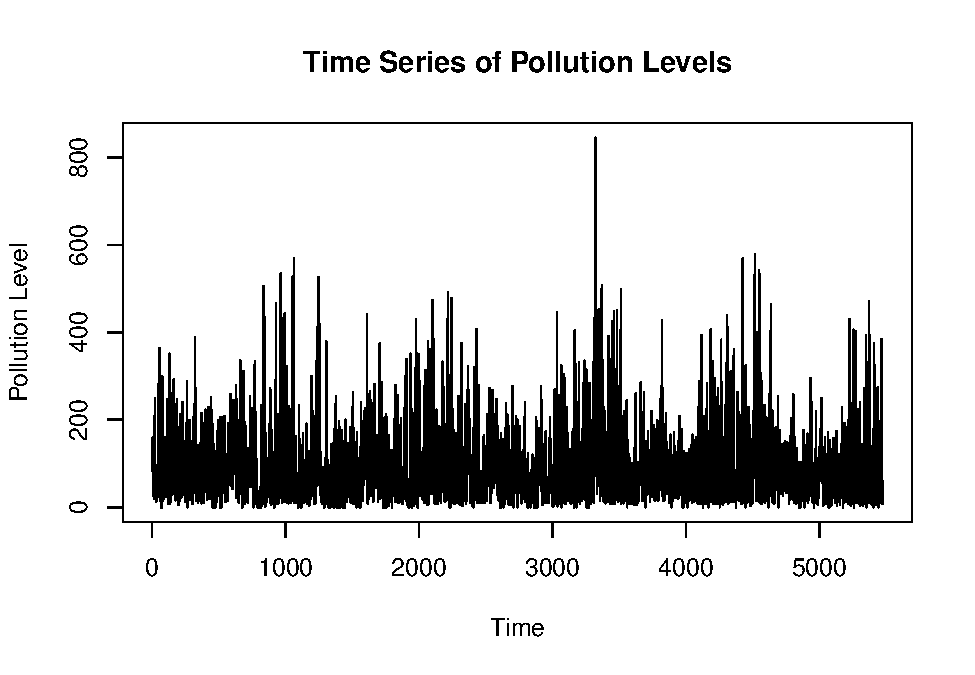
\includegraphics{Final-Project_files/figure-latex/2.2.1-1.pdf}

\subsection{Step 2: Transformation}\label{step-2-transformation}

\begin{Shaded}
\begin{Highlighting}[]
\NormalTok{df}\SpecialCharTok{$}\NormalTok{pollution\_log }\OtherTok{\textless{}{-}} \FunctionTok{log}\NormalTok{(df}\SpecialCharTok{$}\NormalTok{pollution }\SpecialCharTok{+} \DecValTok{1}\NormalTok{)}

\FunctionTok{plot.ts}\NormalTok{(df}\SpecialCharTok{$}\NormalTok{pollution\_log, }\AttributeTok{main=}\StringTok{"Log Transformed Pollution Data"}\NormalTok{,}
        \AttributeTok{ylab=}\StringTok{"Log Transformed Pollution Level"}\NormalTok{, }\AttributeTok{xlab=}\StringTok{"Time"}\NormalTok{)}
\end{Highlighting}
\end{Shaded}

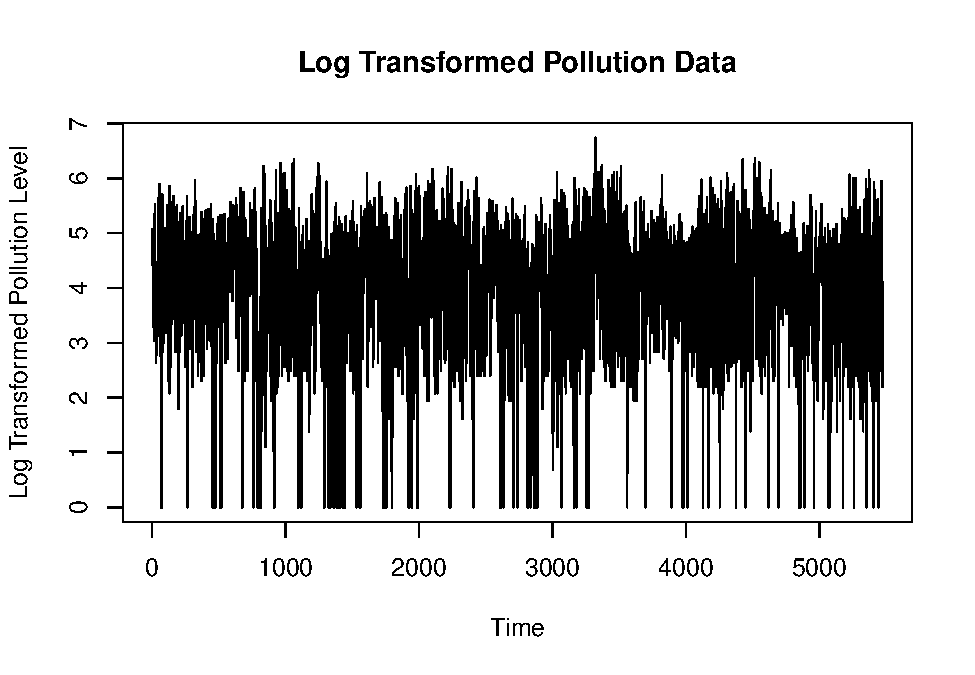
\includegraphics{Final-Project_files/figure-latex/2.1.2-1.pdf}

\subsection{Step 3: Identification}\label{step-3-identification}

\begin{Shaded}
\begin{Highlighting}[]
\FunctionTok{library}\NormalTok{(forecast)}
\FunctionTok{library}\NormalTok{(tseries)}
\FunctionTok{par}\NormalTok{(}\AttributeTok{mfrow=}\FunctionTok{c}\NormalTok{(}\DecValTok{1}\NormalTok{,}\DecValTok{2}\NormalTok{))}

\FunctionTok{acf}\NormalTok{(df}\SpecialCharTok{$}\NormalTok{pollution\_log, }\AttributeTok{main=}\StringTok{"ACF of Log Transformed Data"}\NormalTok{)}
\FunctionTok{pacf}\NormalTok{(df}\SpecialCharTok{$}\NormalTok{pollution\_log, }\AttributeTok{main=}\StringTok{"PACF of Log Transformed Data"}\NormalTok{)}
\end{Highlighting}
\end{Shaded}

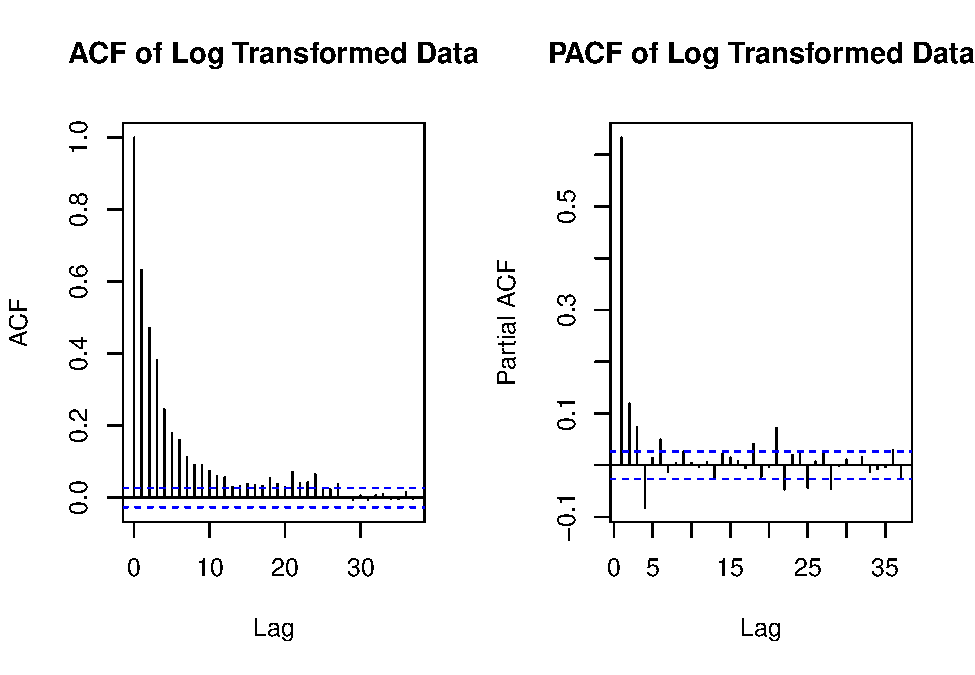
\includegraphics{Final-Project_files/figure-latex/2.1.3-1.pdf}

\begin{Shaded}
\begin{Highlighting}[]
\FunctionTok{par}\NormalTok{(}\AttributeTok{mfrow=}\FunctionTok{c}\NormalTok{(}\DecValTok{1}\NormalTok{,}\DecValTok{1}\NormalTok{))}

\FunctionTok{adf.test}\NormalTok{(df}\SpecialCharTok{$}\NormalTok{pollution\_log)}
\end{Highlighting}
\end{Shaded}

\begin{verbatim}
## 
##  Augmented Dickey-Fuller Test
## 
## data:  df$pollution_log
## Dickey-Fuller = -14.066, Lag order = 17, p-value = 0.01
## alternative hypothesis: stationary
\end{verbatim}

\subsection{Step 4: Estimation of
parameters}\label{step-4-estimation-of-parameters}

\begin{Shaded}
\begin{Highlighting}[]
\FunctionTok{library}\NormalTok{(astsa)}
\end{Highlighting}
\end{Shaded}

\begin{verbatim}
## 
## 载入程辑包：'astsa'
\end{verbatim}

\begin{verbatim}
## The following object is masked from 'package:forecast':
## 
##     gas
\end{verbatim}

\begin{Shaded}
\begin{Highlighting}[]
\NormalTok{fit }\OtherTok{\textless{}{-}} \FunctionTok{sarima}\NormalTok{(df}\SpecialCharTok{$}\NormalTok{pollution\_log, }\AttributeTok{p=}\DecValTok{3}\NormalTok{, }\AttributeTok{d=}\DecValTok{0}\NormalTok{, }\AttributeTok{q=}\DecValTok{2}\NormalTok{)}
\end{Highlighting}
\end{Shaded}

\begin{verbatim}
## initial  value 0.283782 
## iter   2 value 0.078433
## iter   3 value 0.029221
## iter   4 value 0.017241
## iter   5 value 0.016198
## iter   6 value 0.016088
## iter   7 value 0.016035
## iter   8 value 0.015730
## iter   9 value 0.015095
## iter  10 value 0.013850
## iter  11 value 0.013514
## iter  12 value 0.013398
## iter  13 value 0.013337
## iter  14 value 0.013325
## iter  15 value 0.013324
## iter  16 value 0.013323
## iter  17 value 0.013322
## iter  18 value 0.013319
## iter  19 value 0.013313
## iter  20 value 0.013307
## iter  21 value 0.013306
## iter  22 value 0.013305
## iter  23 value 0.013305
## iter  24 value 0.013305
## iter  25 value 0.013305
## iter  26 value 0.013304
## iter  27 value 0.013304
## iter  28 value 0.013304
## iter  29 value 0.013304
## iter  29 value 0.013304
## iter  29 value 0.013304
## final  value 0.013304 
## converged
## initial  value 0.013170 
## iter   2 value 0.013170
## iter   3 value 0.013170
## iter   4 value 0.013170
## iter   5 value 0.013170
## iter   6 value 0.013170
## iter   7 value 0.013170
## iter   8 value 0.013170
## iter   8 value 0.013170
## iter   8 value 0.013170
## final  value 0.013170 
## converged
## <><><><><><><><><><><><><><>
##  
## Coefficients: 
##       Estimate     SE t.value p.value
## ar1     0.0623 0.0748  0.8322  0.4053
## ar2    -0.0962 0.0600 -1.6043  0.1087
## ar3     0.4119 0.0360 11.4350  0.0000
## ma1     0.4959 0.0787  6.2996  0.0000
## ma2     0.4585 0.0602  7.6218  0.0000
## xmean   3.9563 0.0430 91.9885  0.0000
## 
## sigma^2 estimated as 1.026576 on 5469 degrees of freedom 
##  
## AIC = 2.866773  AICc = 2.866776  BIC = 2.875222 
## 
\end{verbatim}

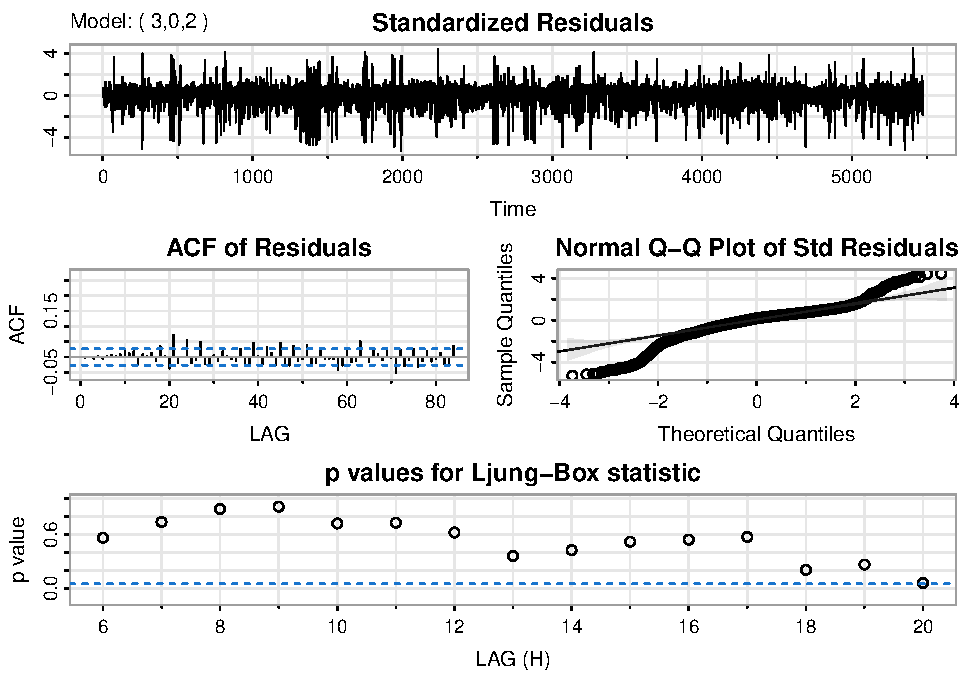
\includegraphics{Final-Project_files/figure-latex/2.1.4-1.pdf}

\subsection{Step 5: Diagnostics}\label{step-5-diagnostics}

\begin{enumerate}
\def\labelenumi{\arabic{enumi}.}
\tightlist
\item
  There is no obvious patterns and no outliers exceeding 3 standard
  deviations.
\item
  The plot of the estimated ACF of the residuals shows nearly no
  apparent departure from the model assumption, except a few lags.
\item
  The normal Q-Q plot of the residuals show that the assumption of
  normality is reasonable, although there are some outliers.
\item
  The Q-statistic is not statistically significant.
\end{enumerate}

\subsection{Step 6: Model selection}\label{step-6-model-selection}

\begin{Shaded}
\begin{Highlighting}[]
\NormalTok{df\_best }\OtherTok{\textless{}{-}} \FunctionTok{auto.arima}\NormalTok{(df}\SpecialCharTok{$}\NormalTok{pollution\_log, }\AttributeTok{seasonal =} \ConstantTok{FALSE}\NormalTok{, }\AttributeTok{ic=}\StringTok{"bic"}\NormalTok{)}
\FunctionTok{summary}\NormalTok{(df\_best)}
\end{Highlighting}
\end{Shaded}

\begin{verbatim}
## Series: df$pollution_log 
## ARIMA(3,0,2) with non-zero mean 
## 
## Coefficients:
##          ar1      ar2     ar3     ma1     ma2    mean
##       0.0623  -0.0962  0.4119  0.4959  0.4585  3.9563
## s.e.  0.0748   0.0600  0.0360  0.0787  0.0602  0.0430
## 
## sigma^2 = 1.028:  log likelihood = -7840.79
## AIC=15695.58   AICc=15695.6   BIC=15741.84
## 
## Training set error measures:
##                         ME     RMSE       MAE  MPE MAPE     MASE       ACF1
## Training set -2.257256e-05 1.013201 0.7233307 -Inf  Inf 1.017692 -0.0018061
\end{verbatim}

ARIMA(3,0,2) is the best selection for this model.

\subsection{Additional Step: Forecast}\label{additional-step-forecast}

\begin{Shaded}
\begin{Highlighting}[]
\NormalTok{df\_forecast }\OtherTok{\textless{}{-}} \FunctionTok{forecast}\NormalTok{(df\_best, }\AttributeTok{h=}\DecValTok{12}\NormalTok{)}
\NormalTok{df\_forecast1 }\OtherTok{\textless{}{-}} \FunctionTok{exp}\NormalTok{(df\_forecast}\SpecialCharTok{$}\NormalTok{mean)}
\NormalTok{df\_forecast1}
\end{Highlighting}
\end{Shaded}

\begin{verbatim}
## Time Series:
## Start = 5476 
## End = 5487 
## Frequency = 1 
##  [1] 15.41574 20.48610 26.86361 33.18135 36.82611 40.61050 44.12829 45.86931
##  [9] 47.48960 49.06628 49.78962 50.39421
\end{verbatim}

\begin{Shaded}
\begin{Highlighting}[]
\NormalTok{time\_index }\OtherTok{\textless{}{-}} \DecValTok{1}\SpecialCharTok{:}\DecValTok{12}
\FunctionTok{plot}\NormalTok{(time\_index, df\_forecast1,}
     \AttributeTok{type =} \StringTok{"o"}\NormalTok{, }\AttributeTok{col =} \StringTok{"blue"}\NormalTok{,}
     \AttributeTok{xlab =} \StringTok{"Forecast Step"}\NormalTok{,}
     \AttributeTok{ylab =} \StringTok{"Pollution Level"}\NormalTok{,}
     \AttributeTok{main =} \StringTok{"12{-}Step Ahead Forecast of Pollution"}\NormalTok{)}
\end{Highlighting}
\end{Shaded}

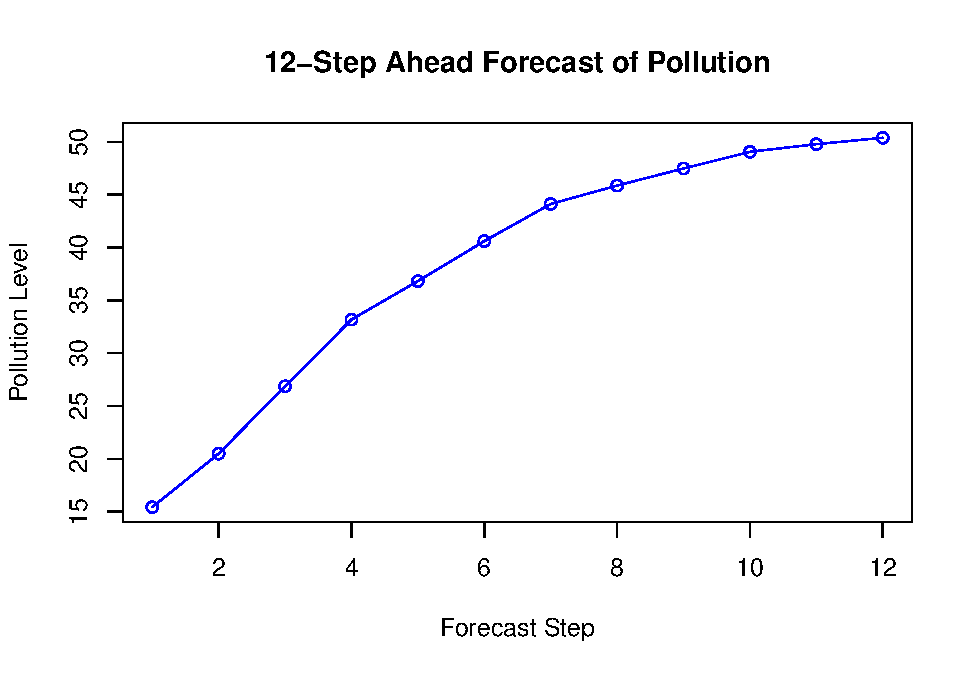
\includegraphics{Final-Project_files/figure-latex/2.2-1.pdf}

\section{Unit Root}\label{unit-root}

\subsection{Step 1: DF Test}\label{step-1-df-test}

\begin{Shaded}
\begin{Highlighting}[]
\NormalTok{df\_result }\OtherTok{\textless{}{-}} \FunctionTok{adf.test}\NormalTok{(df}\SpecialCharTok{$}\NormalTok{pollution\_log, }\AttributeTok{k =} \DecValTok{0}\NormalTok{)}
\end{Highlighting}
\end{Shaded}

\begin{verbatim}
## Warning in adf.test(df$pollution_log, k = 0): p-value smaller than printed p-
## value
\end{verbatim}

\begin{Shaded}
\begin{Highlighting}[]
\FunctionTok{print}\NormalTok{(df\_result)}
\end{Highlighting}
\end{Shaded}

\begin{verbatim}
## 
##  Augmented Dickey-Fuller Test
## 
## data:  df$pollution_log
## Dickey-Fuller = -35.097, Lag order = 0, p-value = 0.01
## alternative hypothesis: stationary
\end{verbatim}

\subsection{Step 2: ADF Test}\label{step-2-adf-test}

\begin{Shaded}
\begin{Highlighting}[]
\NormalTok{adf\_result }\OtherTok{\textless{}{-}} \FunctionTok{adf.test}\NormalTok{(df}\SpecialCharTok{$}\NormalTok{pollution\_log)}
\end{Highlighting}
\end{Shaded}

\begin{verbatim}
## Warning in adf.test(df$pollution_log): p-value smaller than printed p-value
\end{verbatim}

\begin{Shaded}
\begin{Highlighting}[]
\FunctionTok{print}\NormalTok{(adf\_result)}
\end{Highlighting}
\end{Shaded}

\begin{verbatim}
## 
##  Augmented Dickey-Fuller Test
## 
## data:  df$pollution_log
## Dickey-Fuller = -14.066, Lag order = 17, p-value = 0.01
## alternative hypothesis: stationary
\end{verbatim}

\subsection{Step 3: PP Test}\label{step-3-pp-test}

\begin{Shaded}
\begin{Highlighting}[]
\NormalTok{pp\_result }\OtherTok{\textless{}{-}} \FunctionTok{pp.test}\NormalTok{(df}\SpecialCharTok{$}\NormalTok{pollution\_log)}
\end{Highlighting}
\end{Shaded}

\begin{verbatim}
## Warning in pp.test(df$pollution_log): p-value smaller than printed p-value
\end{verbatim}

\begin{Shaded}
\begin{Highlighting}[]
\FunctionTok{print}\NormalTok{(pp\_result)}
\end{Highlighting}
\end{Shaded}

\begin{verbatim}
## 
##  Phillips-Perron Unit Root Test
## 
## data:  df$pollution_log
## Dickey-Fuller Z(alpha) = -2257.2, Truncation lag parameter = 10,
## p-value = 0.01
## alternative hypothesis: stationary
\end{verbatim}

\section{ARMAX Method}\label{armax-method}

\subsection{Selection criteria}\label{selection-criteria}

\begin{Shaded}
\begin{Highlighting}[]
\FunctionTok{library}\NormalTok{(vars)}
\NormalTok{dfvars }\OtherTok{\textless{}{-}} \FunctionTok{cbind}\NormalTok{(}\AttributeTok{pollution\_log =}\NormalTok{ df}\SpecialCharTok{$}\NormalTok{pollution\_log,}
                   \AttributeTok{TEMP =}\NormalTok{ df}\SpecialCharTok{$}\NormalTok{temp,}
                   \AttributeTok{DEW =}\NormalTok{ df}\SpecialCharTok{$}\NormalTok{dew,}
                   \AttributeTok{PRESS =}\NormalTok{ df}\SpecialCharTok{$}\NormalTok{press)}

\NormalTok{dfvars }\OtherTok{\textless{}{-}} \FunctionTok{na.omit}\NormalTok{(dfvars)}
\FunctionTok{VARselect}\NormalTok{(dfvars, }\AttributeTok{lag.max =} \DecValTok{10}\NormalTok{, }\AttributeTok{type =} \StringTok{"both"}\NormalTok{)}
\end{Highlighting}
\end{Shaded}

\begin{verbatim}
## $selection
## AIC(n)  HQ(n)  SC(n) FPE(n) 
##     10     10     10     10 
## 
## $criteria
##                  1           2          3          4          5          6
## AIC(n)    7.445296    7.022673   6.006787   5.848057   5.785693   5.722004
## HQ(n)     7.455418    7.039543   6.030406   5.878424   5.822809   5.765868
## SC(n)     7.474307    7.071025   6.074480   5.935091   5.892068   5.847720
## FPE(n) 1711.791789 1121.780740 406.176336 346.560403 325.607721 305.516801
##                 7          8          9         10
## AIC(n)   5.681481   5.653553   5.626481   5.606281
## HQ(n)    5.732092   5.710913   5.690589   5.677138
## SC(n)    5.826537   5.817950   5.810219   5.809360
## FPE(n) 293.383641 285.303468 277.683444 272.130677
\end{verbatim}

\begin{Shaded}
\begin{Highlighting}[]
\NormalTok{dfarmax }\OtherTok{\textless{}{-}} \FunctionTok{VAR}\NormalTok{(dfvars, }\AttributeTok{p =} \DecValTok{2}\NormalTok{, }\AttributeTok{type =} \StringTok{"both"}\NormalTok{)}
\FunctionTok{summary}\NormalTok{(dfarmax)}
\end{Highlighting}
\end{Shaded}

\begin{verbatim}
## 
## VAR Estimation Results:
## ========================= 
## Endogenous variables: pollution_log, TEMP, DEW, PRESS 
## Deterministic variables: both 
## Sample size: 5473 
## Log Likelihood: -50244.35 
## Roots of the characteristic polynomial:
## 0.9859 0.8228 0.6635 0.6635 0.2761 0.2761 0.2634 0.2098
## Call:
## VAR(y = dfvars, p = 2, type = "both")
## 
## 
## Estimation results for equation pollution_log: 
## ============================================== 
## pollution_log = pollution_log.l1 + TEMP.l1 + DEW.l1 + PRESS.l1 + pollution_log.l2 + TEMP.l2 + DEW.l2 + PRESS.l2 + const + trend 
## 
##                    Estimate Std. Error t value Pr(>|t|)    
## pollution_log.l1  5.166e-01  1.466e-02  35.246  < 2e-16 ***
## TEMP.l1           7.685e-03  3.589e-03   2.141  0.03228 *  
## DEW.l1            1.640e-02  3.930e-03   4.173 3.05e-05 ***
## PRESS.l1         -6.353e-02  5.968e-03 -10.645  < 2e-16 ***
## pollution_log.l2  1.693e-01  1.448e-02  11.693  < 2e-16 ***
## TEMP.l2           1.045e-02  3.503e-03   2.983  0.00286 ** 
## DEW.l2           -2.416e-02  4.000e-03  -6.041 1.64e-09 ***
## PRESS.l2          7.530e-02  5.927e-03  12.704  < 2e-16 ***
## const            -1.095e+01  2.697e+00  -4.060 4.97e-05 ***
## trend             6.133e-06  8.597e-06   0.713  0.47560    
## ---
## Signif. codes:  0 '***' 0.001 '**' 0.01 '*' 0.05 '.' 0.1 ' ' 1
## 
## 
## Residual standard error: 0.9934 on 5463 degrees of freedom
## Multiple R-Squared: 0.4416,  Adjusted R-squared: 0.4407 
## F-statistic:   480 on 9 and 5463 DF,  p-value: < 2.2e-16 
## 
## 
## Estimation results for equation TEMP: 
## ===================================== 
## TEMP = pollution_log.l1 + TEMP.l1 + DEW.l1 + PRESS.l1 + pollution_log.l2 + TEMP.l2 + DEW.l2 + PRESS.l2 + const + trend 
## 
##                    Estimate Std. Error t value Pr(>|t|)    
## pollution_log.l1 -3.158e-01  7.269e-02  -4.345 1.42e-05 ***
## TEMP.l1           4.818e-01  1.780e-02  27.073  < 2e-16 ***
## DEW.l1            3.767e-01  1.949e-02  19.331  < 2e-16 ***
## PRESS.l1          4.536e-01  2.960e-02  15.326  < 2e-16 ***
## pollution_log.l2 -1.460e-01  7.179e-02  -2.033   0.0421 *  
## TEMP.l2          -3.423e-02  1.737e-02  -1.971   0.0488 *  
## DEW.l2           -3.135e-02  1.984e-02  -1.580   0.1141    
## PRESS.l2         -6.038e-01  2.939e-02 -20.541  < 2e-16 ***
## const             1.603e+02  1.337e+01  11.985  < 2e-16 ***
## trend             1.726e-04  4.263e-05   4.050 5.19e-05 ***
## ---
## Signif. codes:  0 '***' 0.001 '**' 0.01 '*' 0.05 '.' 0.1 ' ' 1
## 
## 
## Residual standard error: 4.926 on 5463 degrees of freedom
## Multiple R-Squared: 0.8403,  Adjusted R-squared:  0.84 
## F-statistic:  3194 on 9 and 5463 DF,  p-value: < 2.2e-16 
## 
## 
## Estimation results for equation DEW: 
## ==================================== 
## DEW = pollution_log.l1 + TEMP.l1 + DEW.l1 + PRESS.l1 + pollution_log.l2 + TEMP.l2 + DEW.l2 + PRESS.l2 + const + trend 
## 
##                    Estimate Std. Error t value Pr(>|t|)    
## pollution_log.l1  2.813e-01  5.534e-02   5.082 3.85e-07 ***
## TEMP.l1           8.084e-02  1.355e-02   5.966 2.58e-09 ***
## DEW.l1            6.547e-01  1.484e-02  44.124  < 2e-16 ***
## PRESS.l1         -4.136e-01  2.253e-02 -18.353  < 2e-16 ***
## pollution_log.l2 -1.725e-01  5.466e-02  -3.156  0.00161 ** 
## TEMP.l2           2.451e-01  1.323e-02  18.530  < 2e-16 ***
## DEW.l2            1.244e-01  1.510e-02   8.235 2.23e-16 ***
## PRESS.l2          5.142e-01  2.238e-02  22.975  < 2e-16 ***
## const            -1.061e+02  1.018e+01 -10.420  < 2e-16 ***
## trend            -9.896e-05  3.246e-05  -3.049  0.00231 ** 
## ---
## Signif. codes:  0 '***' 0.001 '**' 0.01 '*' 0.05 '.' 0.1 ' ' 1
## 
## 
## Residual standard error: 3.75 on 5463 degrees of freedom
## Multiple R-Squared: 0.9327,  Adjusted R-squared: 0.9326 
## F-statistic:  8418 on 9 and 5463 DF,  p-value: < 2.2e-16 
## 
## 
## Estimation results for equation PRESS: 
## ====================================== 
## PRESS = pollution_log.l1 + TEMP.l1 + DEW.l1 + PRESS.l1 + pollution_log.l2 + TEMP.l2 + DEW.l2 + PRESS.l2 + const + trend 
## 
##                    Estimate Std. Error t value Pr(>|t|)    
## pollution_log.l1  1.133e-01  4.409e-02   2.569  0.01021 *  
## TEMP.l1           1.300e-01  1.080e-02  12.037  < 2e-16 ***
## DEW.l1           -1.725e-01  1.182e-02 -14.590  < 2e-16 ***
## PRESS.l1          1.044e+00  1.795e-02  58.168  < 2e-16 ***
## pollution_log.l2  1.320e-01  4.355e-02   3.032  0.00244 ** 
## TEMP.l2          -5.147e-04  1.054e-02  -0.049  0.96104    
## DEW.l2            3.692e-02  1.203e-02   3.068  0.00217 ** 
## PRESS.l2         -1.108e-01  1.783e-02  -6.214 5.54e-10 ***
## const             6.532e+01  8.113e+00   8.052 9.92e-16 ***
## trend            -3.753e-05  2.586e-05  -1.451  0.14672    
## ---
## Signif. codes:  0 '***' 0.001 '**' 0.01 '*' 0.05 '.' 0.1 ' ' 1
## 
## 
## Residual standard error: 2.988 on 5463 degrees of freedom
## Multiple R-Squared: 0.9157,  Adjusted R-squared: 0.9156 
## F-statistic:  6595 on 9 and 5463 DF,  p-value: < 2.2e-16 
## 
## 
## 
## Covariance matrix of residuals:
##               pollution_log     TEMP     DEW    PRESS
## pollution_log        0.9868  -0.5648  1.5559  -0.2490
## TEMP                -0.5648  24.2654 -4.4531 -10.1700
## DEW                  1.5559  -4.4531 14.0662  -0.2167
## PRESS               -0.2490 -10.1700 -0.2167   8.9297
## 
## Correlation matrix of residuals:
##               pollution_log    TEMP      DEW    PRESS
## pollution_log       1.00000 -0.1154  0.41763 -0.08389
## TEMP               -0.11542  1.0000 -0.24104 -0.69089
## DEW                 0.41763 -0.2410  1.00000 -0.01934
## PRESS              -0.08389 -0.6909 -0.01934  1.00000
\end{verbatim}

\begin{Shaded}
\begin{Highlighting}[]
\NormalTok{dfarmax }\OtherTok{\textless{}{-}} \FunctionTok{VAR}\NormalTok{(dfvars, }\AttributeTok{p =} \DecValTok{2}\NormalTok{, }\AttributeTok{type =} \StringTok{"both"}\NormalTok{)}
\FunctionTok{summary}\NormalTok{(dfarmax)}
\end{Highlighting}
\end{Shaded}

\begin{verbatim}
## 
## VAR Estimation Results:
## ========================= 
## Endogenous variables: pollution_log, TEMP, DEW, PRESS 
## Deterministic variables: both 
## Sample size: 5473 
## Log Likelihood: -50244.35 
## Roots of the characteristic polynomial:
## 0.9859 0.8228 0.6635 0.6635 0.2761 0.2761 0.2634 0.2098
## Call:
## VAR(y = dfvars, p = 2, type = "both")
## 
## 
## Estimation results for equation pollution_log: 
## ============================================== 
## pollution_log = pollution_log.l1 + TEMP.l1 + DEW.l1 + PRESS.l1 + pollution_log.l2 + TEMP.l2 + DEW.l2 + PRESS.l2 + const + trend 
## 
##                    Estimate Std. Error t value Pr(>|t|)    
## pollution_log.l1  5.166e-01  1.466e-02  35.246  < 2e-16 ***
## TEMP.l1           7.685e-03  3.589e-03   2.141  0.03228 *  
## DEW.l1            1.640e-02  3.930e-03   4.173 3.05e-05 ***
## PRESS.l1         -6.353e-02  5.968e-03 -10.645  < 2e-16 ***
## pollution_log.l2  1.693e-01  1.448e-02  11.693  < 2e-16 ***
## TEMP.l2           1.045e-02  3.503e-03   2.983  0.00286 ** 
## DEW.l2           -2.416e-02  4.000e-03  -6.041 1.64e-09 ***
## PRESS.l2          7.530e-02  5.927e-03  12.704  < 2e-16 ***
## const            -1.095e+01  2.697e+00  -4.060 4.97e-05 ***
## trend             6.133e-06  8.597e-06   0.713  0.47560    
## ---
## Signif. codes:  0 '***' 0.001 '**' 0.01 '*' 0.05 '.' 0.1 ' ' 1
## 
## 
## Residual standard error: 0.9934 on 5463 degrees of freedom
## Multiple R-Squared: 0.4416,  Adjusted R-squared: 0.4407 
## F-statistic:   480 on 9 and 5463 DF,  p-value: < 2.2e-16 
## 
## 
## Estimation results for equation TEMP: 
## ===================================== 
## TEMP = pollution_log.l1 + TEMP.l1 + DEW.l1 + PRESS.l1 + pollution_log.l2 + TEMP.l2 + DEW.l2 + PRESS.l2 + const + trend 
## 
##                    Estimate Std. Error t value Pr(>|t|)    
## pollution_log.l1 -3.158e-01  7.269e-02  -4.345 1.42e-05 ***
## TEMP.l1           4.818e-01  1.780e-02  27.073  < 2e-16 ***
## DEW.l1            3.767e-01  1.949e-02  19.331  < 2e-16 ***
## PRESS.l1          4.536e-01  2.960e-02  15.326  < 2e-16 ***
## pollution_log.l2 -1.460e-01  7.179e-02  -2.033   0.0421 *  
## TEMP.l2          -3.423e-02  1.737e-02  -1.971   0.0488 *  
## DEW.l2           -3.135e-02  1.984e-02  -1.580   0.1141    
## PRESS.l2         -6.038e-01  2.939e-02 -20.541  < 2e-16 ***
## const             1.603e+02  1.337e+01  11.985  < 2e-16 ***
## trend             1.726e-04  4.263e-05   4.050 5.19e-05 ***
## ---
## Signif. codes:  0 '***' 0.001 '**' 0.01 '*' 0.05 '.' 0.1 ' ' 1
## 
## 
## Residual standard error: 4.926 on 5463 degrees of freedom
## Multiple R-Squared: 0.8403,  Adjusted R-squared:  0.84 
## F-statistic:  3194 on 9 and 5463 DF,  p-value: < 2.2e-16 
## 
## 
## Estimation results for equation DEW: 
## ==================================== 
## DEW = pollution_log.l1 + TEMP.l1 + DEW.l1 + PRESS.l1 + pollution_log.l2 + TEMP.l2 + DEW.l2 + PRESS.l2 + const + trend 
## 
##                    Estimate Std. Error t value Pr(>|t|)    
## pollution_log.l1  2.813e-01  5.534e-02   5.082 3.85e-07 ***
## TEMP.l1           8.084e-02  1.355e-02   5.966 2.58e-09 ***
## DEW.l1            6.547e-01  1.484e-02  44.124  < 2e-16 ***
## PRESS.l1         -4.136e-01  2.253e-02 -18.353  < 2e-16 ***
## pollution_log.l2 -1.725e-01  5.466e-02  -3.156  0.00161 ** 
## TEMP.l2           2.451e-01  1.323e-02  18.530  < 2e-16 ***
## DEW.l2            1.244e-01  1.510e-02   8.235 2.23e-16 ***
## PRESS.l2          5.142e-01  2.238e-02  22.975  < 2e-16 ***
## const            -1.061e+02  1.018e+01 -10.420  < 2e-16 ***
## trend            -9.896e-05  3.246e-05  -3.049  0.00231 ** 
## ---
## Signif. codes:  0 '***' 0.001 '**' 0.01 '*' 0.05 '.' 0.1 ' ' 1
## 
## 
## Residual standard error: 3.75 on 5463 degrees of freedom
## Multiple R-Squared: 0.9327,  Adjusted R-squared: 0.9326 
## F-statistic:  8418 on 9 and 5463 DF,  p-value: < 2.2e-16 
## 
## 
## Estimation results for equation PRESS: 
## ====================================== 
## PRESS = pollution_log.l1 + TEMP.l1 + DEW.l1 + PRESS.l1 + pollution_log.l2 + TEMP.l2 + DEW.l2 + PRESS.l2 + const + trend 
## 
##                    Estimate Std. Error t value Pr(>|t|)    
## pollution_log.l1  1.133e-01  4.409e-02   2.569  0.01021 *  
## TEMP.l1           1.300e-01  1.080e-02  12.037  < 2e-16 ***
## DEW.l1           -1.725e-01  1.182e-02 -14.590  < 2e-16 ***
## PRESS.l1          1.044e+00  1.795e-02  58.168  < 2e-16 ***
## pollution_log.l2  1.320e-01  4.355e-02   3.032  0.00244 ** 
## TEMP.l2          -5.147e-04  1.054e-02  -0.049  0.96104    
## DEW.l2            3.692e-02  1.203e-02   3.068  0.00217 ** 
## PRESS.l2         -1.108e-01  1.783e-02  -6.214 5.54e-10 ***
## const             6.532e+01  8.113e+00   8.052 9.92e-16 ***
## trend            -3.753e-05  2.586e-05  -1.451  0.14672    
## ---
## Signif. codes:  0 '***' 0.001 '**' 0.01 '*' 0.05 '.' 0.1 ' ' 1
## 
## 
## Residual standard error: 2.988 on 5463 degrees of freedom
## Multiple R-Squared: 0.9157,  Adjusted R-squared: 0.9156 
## F-statistic:  6595 on 9 and 5463 DF,  p-value: < 2.2e-16 
## 
## 
## 
## Covariance matrix of residuals:
##               pollution_log     TEMP     DEW    PRESS
## pollution_log        0.9868  -0.5648  1.5559  -0.2490
## TEMP                -0.5648  24.2654 -4.4531 -10.1700
## DEW                  1.5559  -4.4531 14.0662  -0.2167
## PRESS               -0.2490 -10.1700 -0.2167   8.9297
## 
## Correlation matrix of residuals:
##               pollution_log    TEMP      DEW    PRESS
## pollution_log       1.00000 -0.1154  0.41763 -0.08389
## TEMP               -0.11542  1.0000 -0.24104 -0.69089
## DEW                 0.41763 -0.2410  1.00000 -0.01934
## PRESS              -0.08389 -0.6909 -0.01934  1.00000
\end{verbatim}

\subsection{Residual ACF/CCF and
Prediction}\label{residual-acfccf-and-prediction}

\begin{Shaded}
\begin{Highlighting}[]
\FunctionTok{serial.test}\NormalTok{(dfarmax, }\AttributeTok{lags.pt =} \DecValTok{12}\NormalTok{, }\AttributeTok{type =} \StringTok{"PT.adjusted"}\NormalTok{)}
\end{Highlighting}
\end{Shaded}

\begin{verbatim}
## 
##  Portmanteau Test (adjusted)
## 
## data:  Residuals of VAR object dfarmax
## Chi-squared = 12950, df = 160, p-value < 2.2e-16
\end{verbatim}

\begin{Shaded}
\begin{Highlighting}[]
\NormalTok{dfpredict }\OtherTok{\textless{}{-}} \FunctionTok{predict}\NormalTok{(dfarmax, }\AttributeTok{n.ahead =} \DecValTok{24}\NormalTok{, }\AttributeTok{ci =} \FloatTok{0.95}\NormalTok{)}
\FunctionTok{fanchart}\NormalTok{(dfpredict)}
\end{Highlighting}
\end{Shaded}

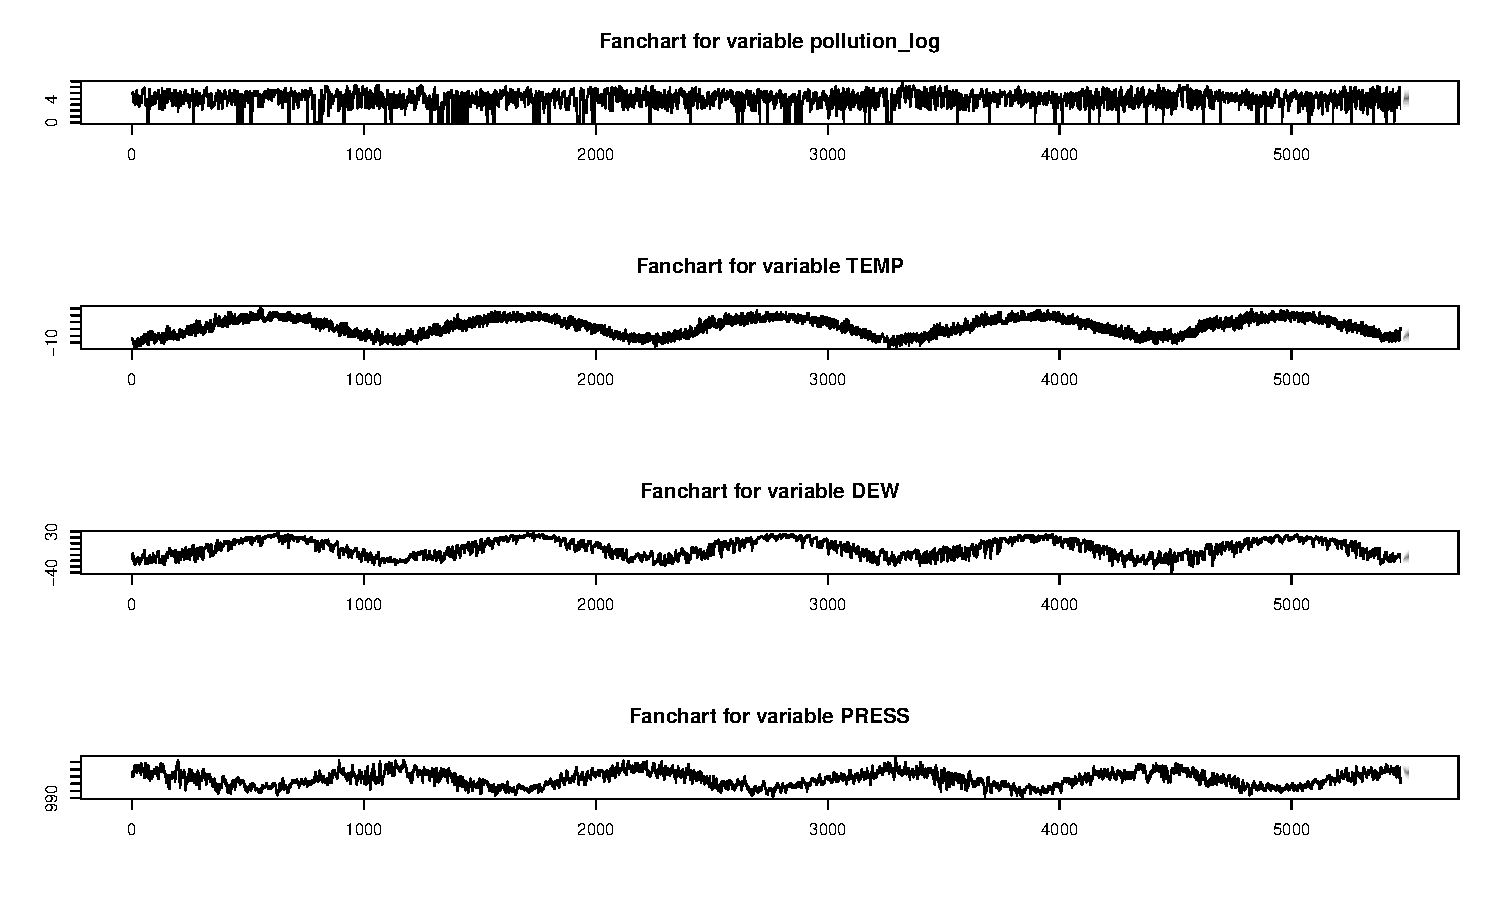
\includegraphics{Final-Project_files/figure-latex/unnamed-chunk-6-1.pdf}

\end{document}
